%\section{پیاده‌سازی کنترل‌کننده \lr{LQDG} بر رویه کانال پیچ}\label{roll_LQDG_section}
%در بخش
%\ref{roll_LQDG_section_simulation}
%شبیه‌سازی تک کانال استند چهارپره در حضور کنترل‌کننده \lr{LQDG} انجام شد.
 در این بخش به پیاده‌سازی کنترل‌کننده \lr{LQDG} بر رویه کانال پیچ استند سه درجه آزادی پرداخته می‌شود.
در پیاده‌سازی از ضرایب وزنی بهینه به دست آمده در قسمت شبیه‌سازی استفاده شده‌است.
\begin{figure}[H]
	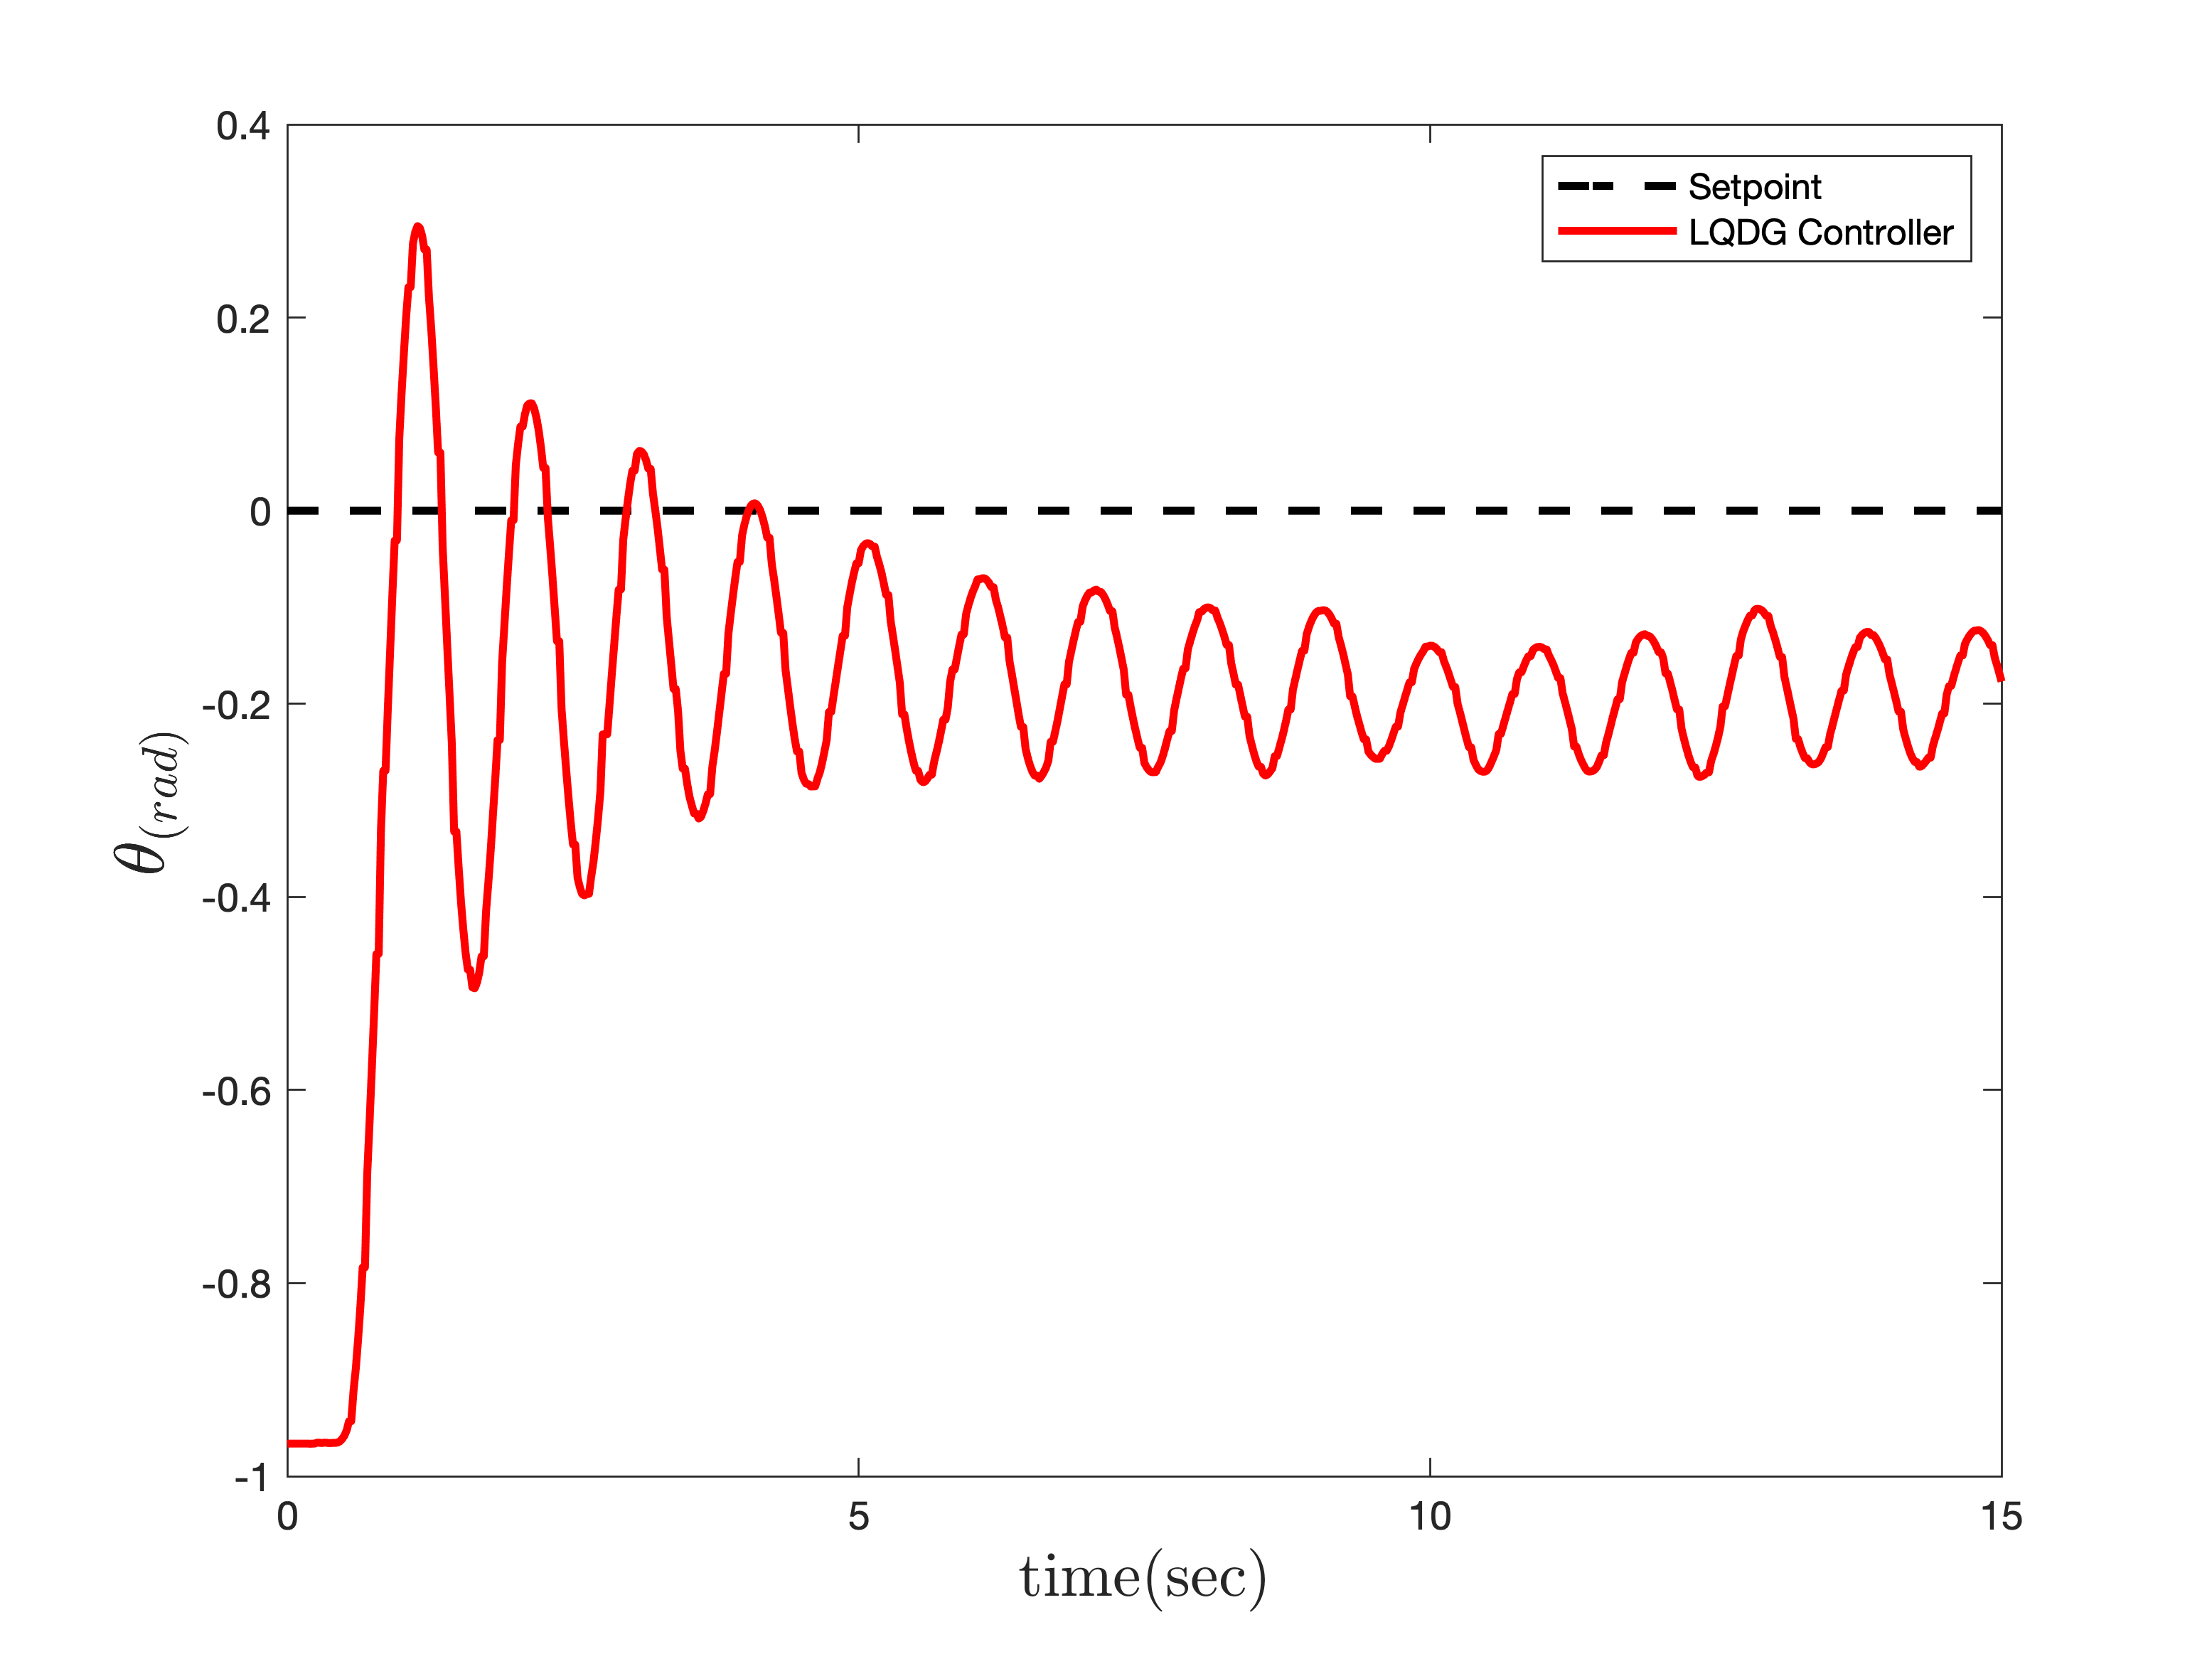
\includegraphics[width=.48\linewidth]{../Figures/Calibration/LQDG/Pitch/lqdg_pitch.png}
	\centering
	\caption{عملكرد کنترل‌کننده \lr{LQDG} در کنترل زاويه پیچ (تعقیب ورودی صفر)}
\end{figure}

\begin{figure}[H]
	\centering
	\subfigure[موتور شماره یک]{
		\centering
		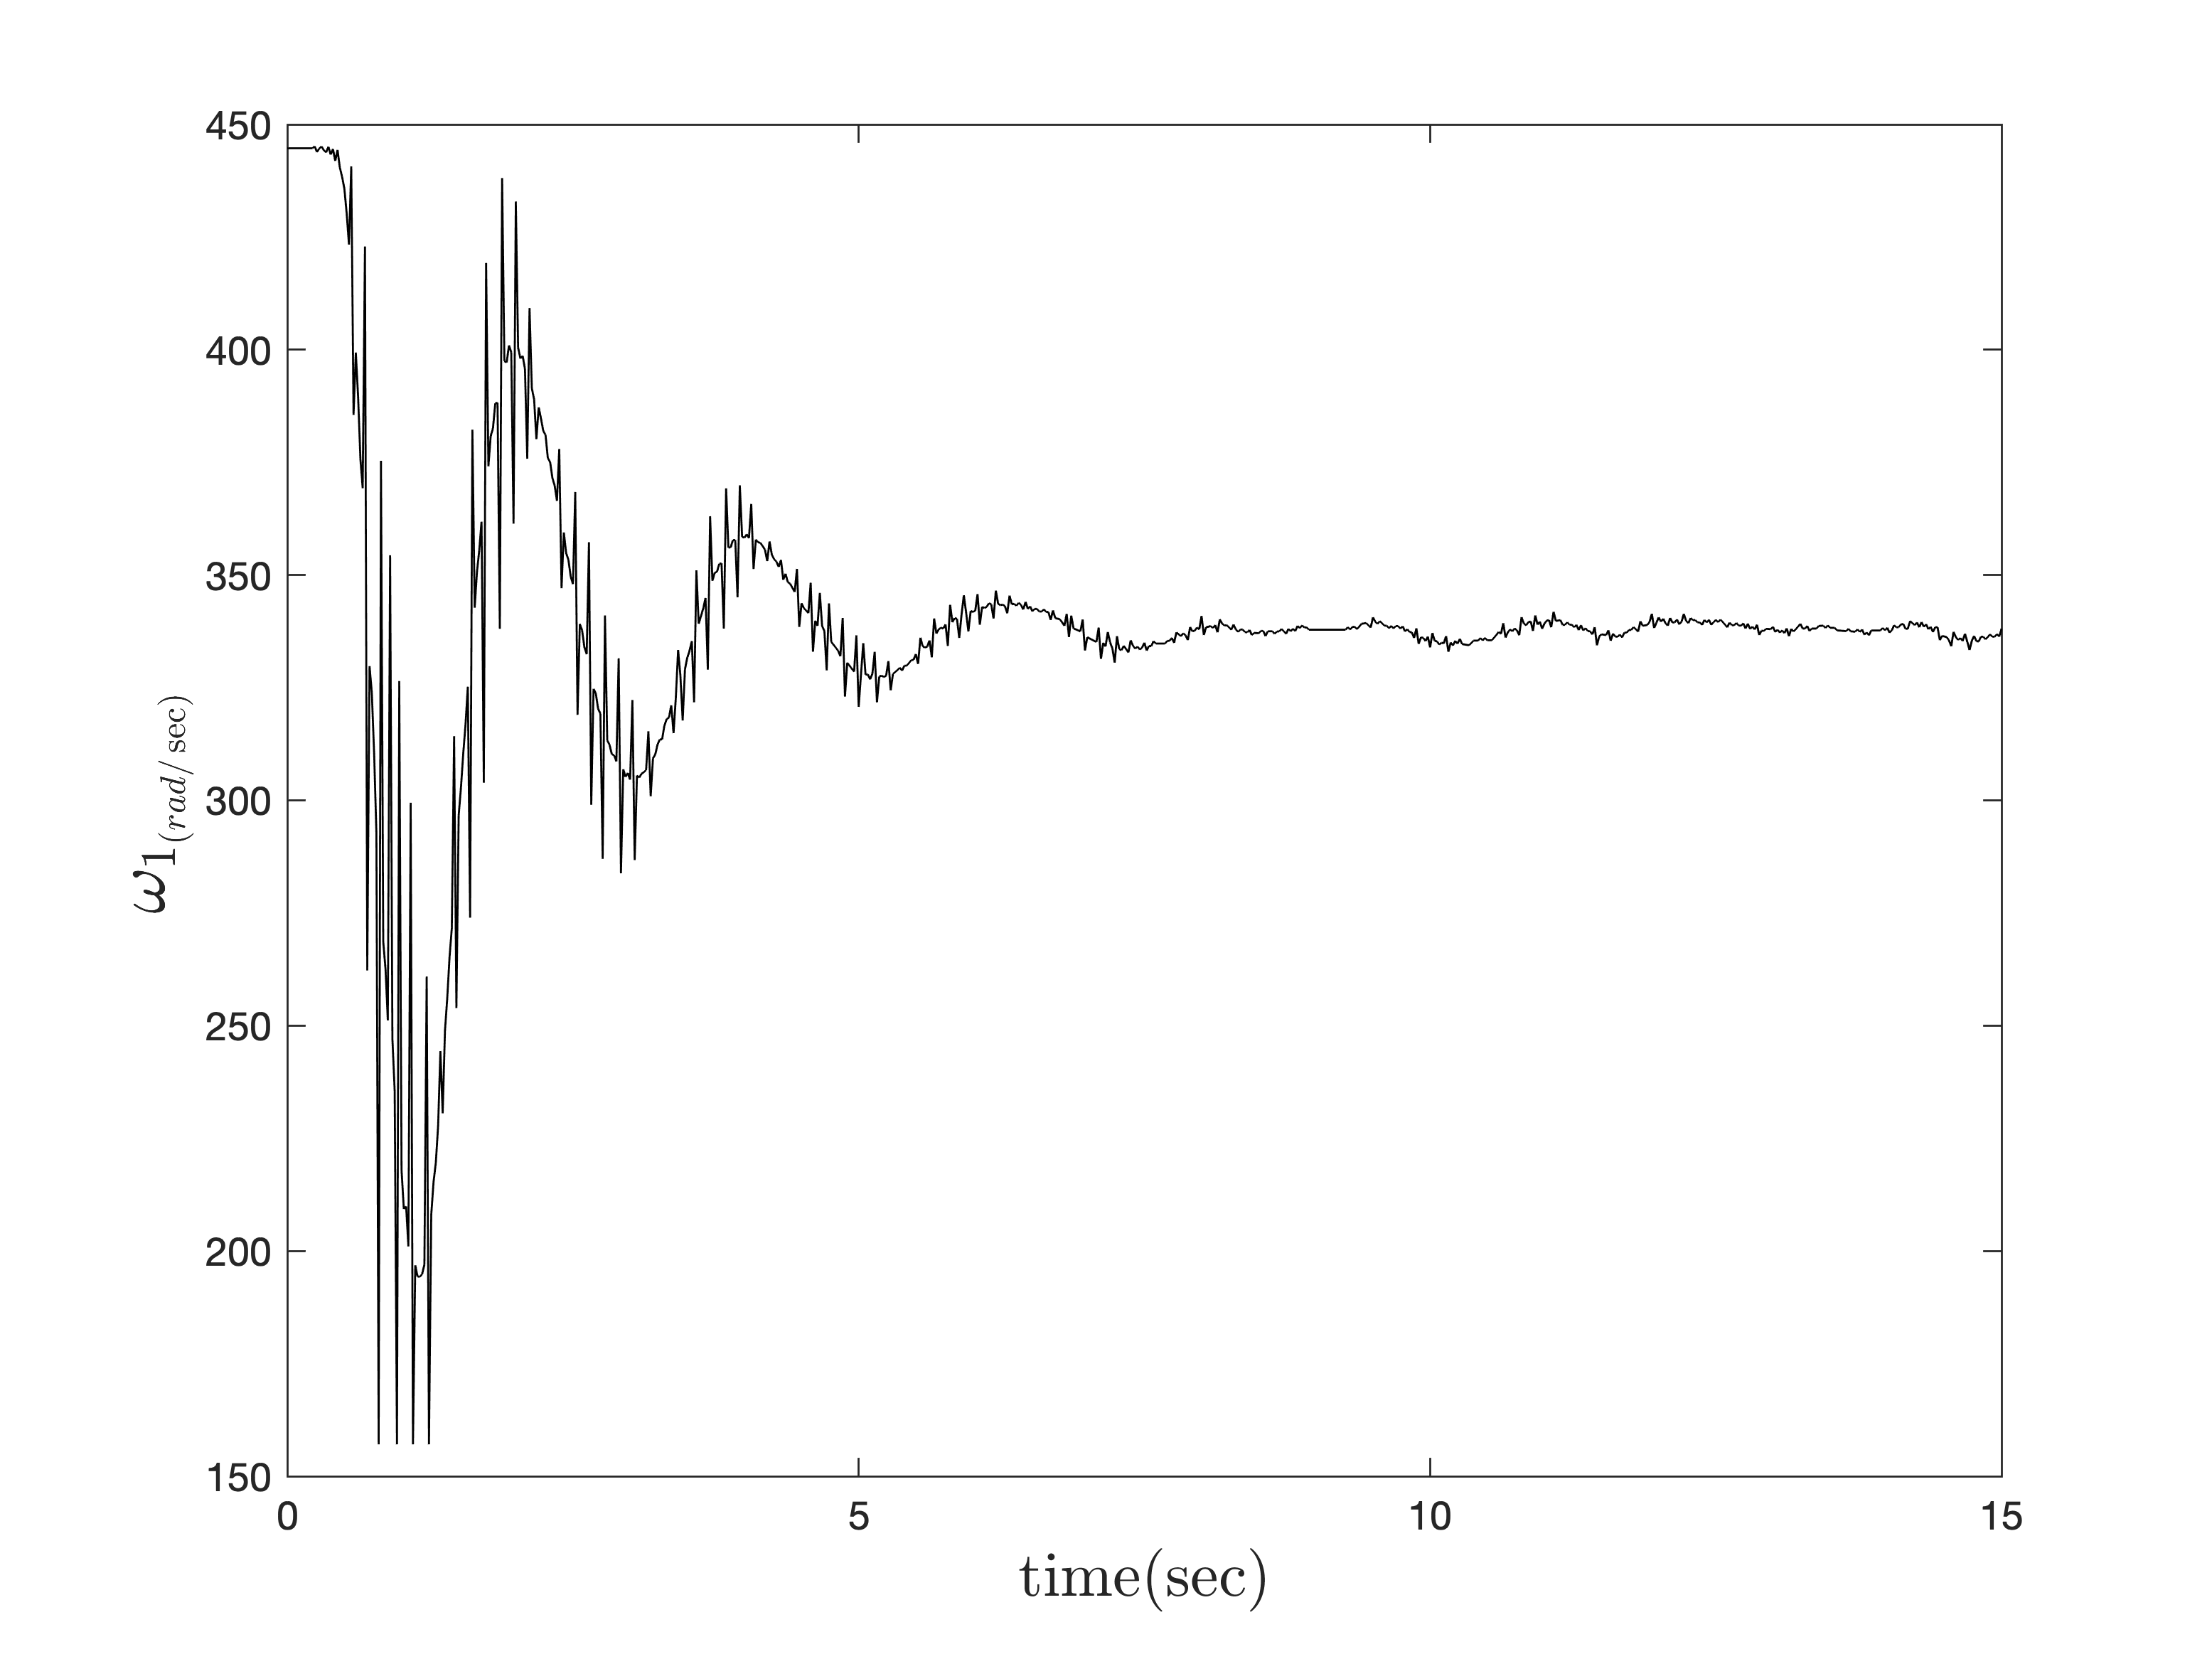
\includegraphics[width=.45\linewidth]{../Figures/Calibration/LQDG/Pitch/lqdg_pitch_Omega_1.png}
	}
	\subfigure[موتور شماره سه]{
		\centering
		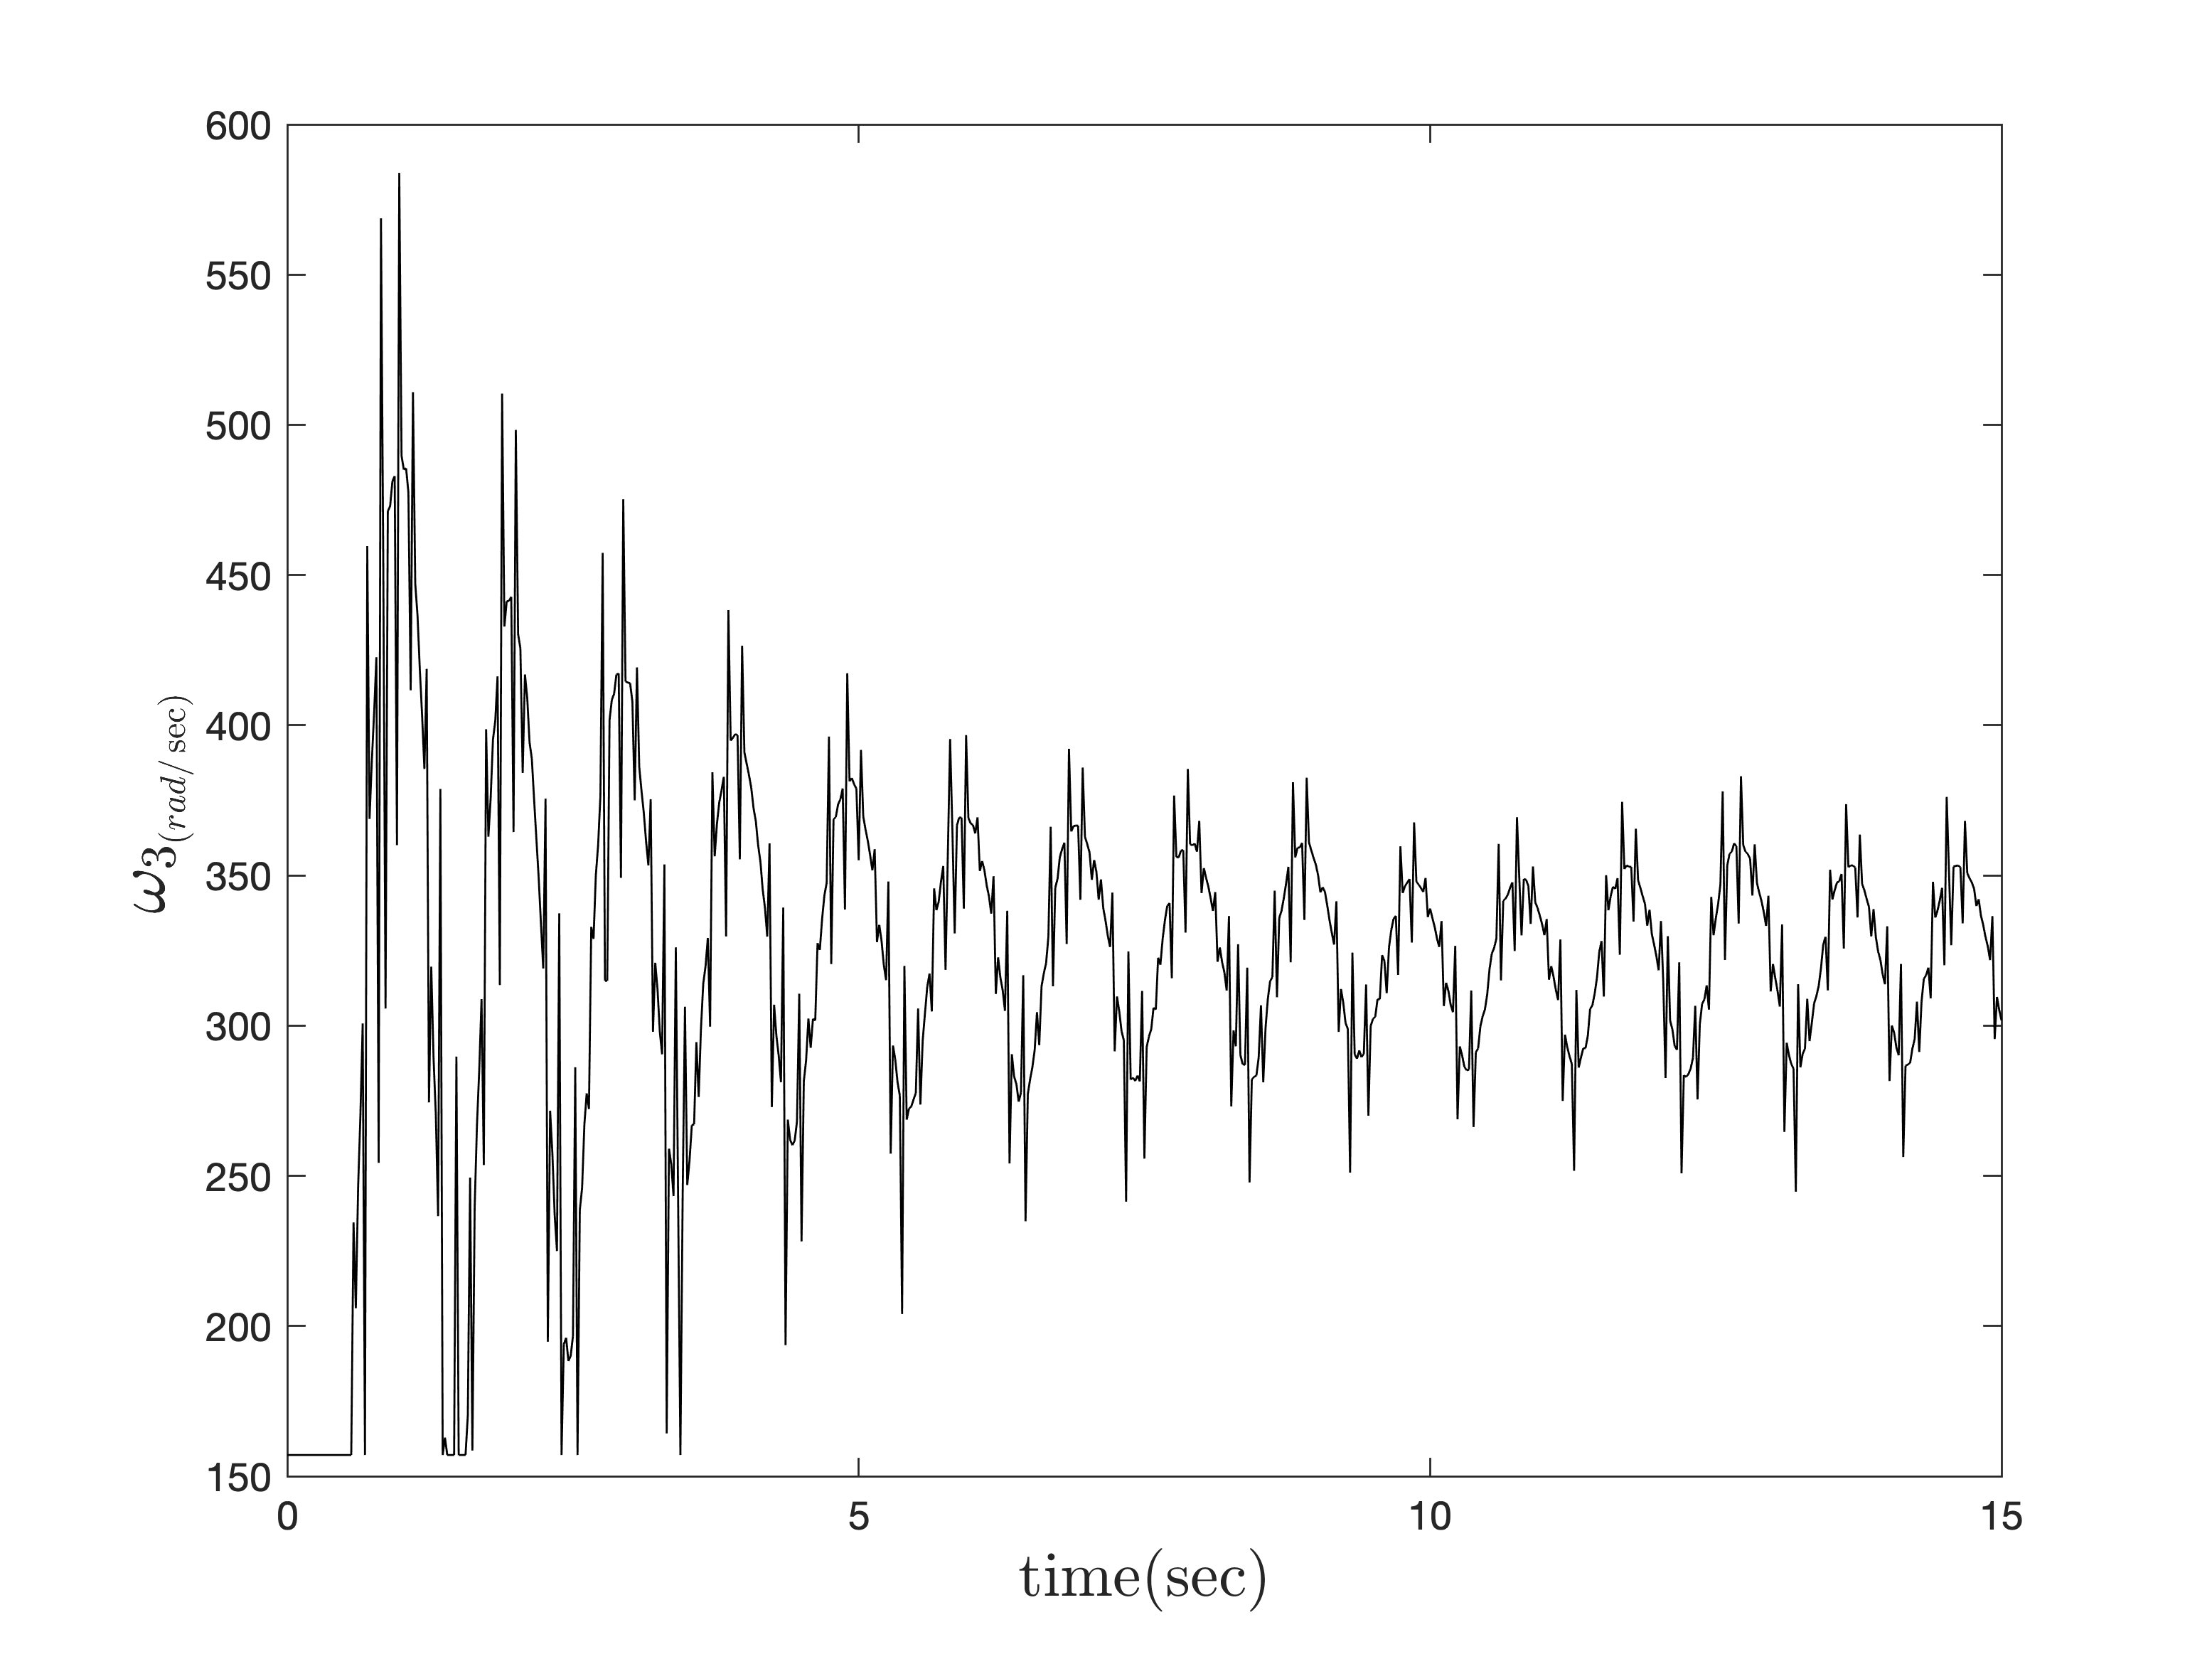
\includegraphics[width=.45\linewidth]{../Figures/Calibration/LQDG/Pitch/lqdg_pitch_Omega_3.png}
	}
	\caption{‫‪فرمان کنترلی موتورهای دو و چهار در کنترل زاویه پیچ (تعقیب ورودی صفر)}
\end{figure}


%بر اساس خروجی شبیه‌سازی (شکل
%\ref{lqdg_roll_fig})
%،کانال رول در حضور کنترل‌کننده \lr{LQDG} در کمتر از پنج ثانیه به تعادل می‌رسد اما دارای خطای ماندگار است ولی خطای مانگار آن نسبت به کنترل‌کننده بخش
%\ref{roll_lqr_section}
%کمتر است. به دلیل خطای ماندگار، در بخش
%%LQIDG
%انتگرال‌گیر به کنترل‌کننده اضافه می‌شود تا خطای مانگار استند را کم کند.
